%-----------------------------------------------------------------------------
% TeX-report 
% Written in LaTeX 2e.
% Work of Dinesh K. Pinto, St. Stephen's College, 2015.
%-----------------------------------------------------------------------------

\documentclass{dkpinto-report}

%---------------------------Title and Page Notes------------------------------
\title{\bfseries Determination of specific rotation of cane sugar using Laurent's half-shade polarimeter} % Title in BOLD
\author{D. Pinto \\ Lab VI-A} % Double backward slash "\\" inserts a new-line 
\date{\vspace{-5ex}} % Reduces vertical space, the date can be added ahead 
\rhead{\textsc{Experiment No.1}} % Right header
\lhead{St. Stephen's College, Delhi} % Left header
%-----------------------------------------------------------------------------

\begin{document}

%-----------------------------Title Page--------------------------------------
\begin{titlepage}
\maketitle 

\begin{center} % Centering environment
\begin{tabular}{r l} % Alignment right(r) and left(l)
Date Performed: & \today \\ 
Instructors: & Prof. A. Gupta \\  
			 & Prof. V. Vyas
\end{tabular}
\end{center}

%\vfill % Add vertical space

\tableofcontents  % Compile twice to view changes 
\thispagestyle{empty}  % Remove pagenumber from titlepage 

\end{titlepage}



%------------------------------Introduction------------------------------------
\section{Introduction} % Numbered section headers
The aim of this experiment is to find the specific rotation of cane sugar using Laurent's half-shade polarimeter.\\
The apparatus used in this experiment is as follows:

\begin{enumerate}  % Numbered list
\itemsep0em  % Reduce item separation
\item Laurent's half-shade polarimeter
\item Sugar solution of concentrations - 5\%, 10\%, 15\%, 20\%, 30\% and 40\%  % The '%' symbol is reserved for comments, to display a %, write it as \%
\item Distilled water
\item Sodium vapour lamp
\item Digital weighing scale
\item Measuring beaker   
\end{enumerate}



%---------------------------------------Theory----------------------------------
\section{Theoretical overview}

\subsection{Linear Polarization}
% Use $...$ for writing inline math relations
Linear polarization or plane polarization of electromagnetic radiation is a confinement of the electric field vector ($\vec{E}$) or magnetic field vector ($\vec{M}$) to a given plane along the direction of propagation. The orientation of a linearly polarized electromagnetic wave is defined by the direction of ($\vec{E}$). The light that is emitted by a Sodium vapor lamp is unpolarized, however, when passed through a Nicol prism, the EM wave emerges as a polarized wave. 

\begin{figure}[h] \label{img:1}  % Begin a figure environment to insert image 
\caption{Linearly polarized light. \texttt{Source:hyperphysics.phy-astr.gsu.edu}} % Add a caption, always cite your sources
\centering  % Center image 
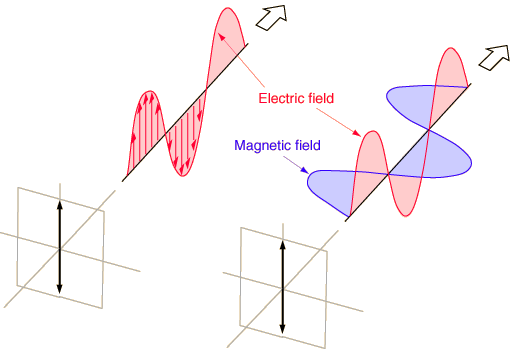
\includegraphics[scale=0.4]{Images/Lin_Pol.png}
\end{figure}

\subsection{The Nicol Prism}
When an ordinary ray of light is passed through a calcite crystal, the non-isotropy of the crystal causes the unpolarized ray to split into two rays:

\begin{itemize} % Bulleted list
\item An \textbf{ordinary ray} which is polarized and has its vibrations perpendicular to the principle section of the crystal;
\item An \textbf{extra-ordinary ray} which is polarized and whose vibration is parallel to the principle section of the prism.
\end{itemize}

In a Nicol prism, the ordinary ray is eliminated and the extra-ordinary ray, which is plane polarized, is transmitted through the prism.

\subsection{Optical rotation}
Substances that are capable of rotating the plane of polarisation of a linearly polarised wave are said to be optically active. In this experiment we study the optical rotation of light by the sugar molecules in a sugar solution. The angle through which the solution rotates the plane of polarisation will depend on,

\begin{enumerate}
\item The concentration of the solution;
\item The thickness of the sample;
\item The wavelength of light; 
\item Temperature.
\end{enumerate}
Assuming that we are holding the temperature of the sample constant and the light is monochromatic we can derive the following relation:

If $x$ grams of sugar are dissolved in volume $V$ (cubic centimeters) of the solution and the length of the tube containing the solution is $l$ decimeter and $\theta$ is the rotation produced, then the specific rotation, $S$ of the cane sugar at the  given temperature and corresponding to the wavelength  is given by 

% For equations, use the the align environment
% \begin{align} will number equations 
% \begn{align*} will NOT number equations
\begin{align*}
S  = \dfrac{\theta}{l} \times \dfrac{v}{x}  = \dfrac{\theta}{lc}
\end{align*}


%-----------------------------Experimental overview-----------------------------------------
\section{Experimental Setup and procedure}

\subsection{Laurent half shade polarimeter}
A polarimeter is a device which is used to measure the optical rotation produced by an optically active substance. It consists of two Nicol prisms capable of rotating about a common axis, and a hollow tube for filling the solution of the optically active substance whose specific rotation is to be determined. It consists of two Nicol prisms, $N_1$ and $N_2$. $N_1$ acts as a polarizer, while $N_2$ acts as an analyzer. Next to $N_1$ there is a half shade device $H$, one half of which is a half wave plate of quartz $Q$ which covers one-half of the field of view while the other half is a glass plate $G$. $T$ is a glass tube having a larger diameter in the middle. The optically active solution is filled in this tube. The larger diameter at the middle ensures that no bubble (which in my experience, there always is) is in the path of the electromagnetic wave. The tube is closed at the ends by cover slips. $N_2$ is capable of rotation about a common axis of $N_1$ and $N_2$. The rotation of the analyzer can be read on a Vernier scale.   

\subsection{Action of the half shade device}
A half-shade device consists of a circular plate of quartz, cut with faces parallel to the optic axis with a thickness such that it acts as a half-wave plate i.e. introduces a path difference of $\lambda / 2$ or a phase difference of $\pi$ between the $E$(extra-ordinary) and $O$(ordinary) vibrations. The other half is made up of a semicircular plate of glass of suitable thickness such that it transmits and absorbs the same amount of light as the quartz plate.

\begin{figure}
\centering
\caption{Half-shade device. \texttt{Source:hyperphysics.phy-astr.gsu.edu}}
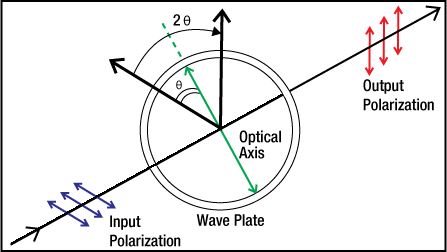
\includegraphics[scale=0.4]{Images/half_plate.png}
\end{figure}

Let the principal plane of Nicol prism $N_1$ be inclined at an angle $\theta$ to the optical axis of the quartz half. On passing through the glass half the vibrations of light remain in the same plane, this is not the case of the quartz half. On passing through the quartz, the beam is split up into the $E$ component along the optic axis of the quartz and the $O$ component perpendicular to the optic axis. On emerging these two components differ in phase by $\pi$, the $O$ component gains a phase of $\pi$ over the $E$ component. Therefore the direction of the $O$ component is now reversed. Now the resultant of the $E$ and the $O$ component will make an angle $\theta$ with the y-axis. Thus the effect of the quartz plate is to rotate the plane of polarization by $2\theta$.  

Thus there are two plane polarized beams, one emerging from the glass half vibrating along $OA$ and the other vibrating along $OC$. 
There are three possible conditions and outcomes,

\begin{enumerate}
\item Principal plane of $N_2 \parallel AOB \implies$ glass half will appear brighter than quartz half; 
\item Principal plane of $N_2 \parallel COD \implies$ quartz half will appear brighter than glass half;
\item Principal plane of $N_2 \parallel YY^{'} \implies$ quartz and glass half are equally bright.
\end{enumerate}

A small change in the angle from position 3 is easily detected by humans, who are quite sensitive to changes in relative brightness. Thus this method can be used to accurately measure the angle of rotation of the plane of polarization using a polarimeter.

%-----------------------------Experimental Procedure---------------------------------
\section{Procedure}

\begin{enumerate}
\itemsep0em
\item A 40 percent sugar solution is prepared. It should contain 40 grams of sugar in 100 cc of the solution with distilled water.
\item Distilled water is filled in the polarimeter tube taking care that no air bubbles are formed.
\item The tube is placed in the polarimeter which is directed towards sodium vapour light. The polariser and half-shade device is kept in a fixed position throughout the experiment.
\item The analyser is rotated till both halves of the half shade device appear equally dark. In an ideal case the angle between the axis of the analyser and polariser should be either 0 or $\pi$.
\item Now the tube filled with the sugar solution is placed in the polarimeter. On looking through the analyser it is observed that the 2 halves are of different intensities. The analyser is rotated till the equally dark condition is met again and the angle of rotation is noted.
\item There will be a small range over which both the halves appear dark. The extrema of this range is noted. i.e. when the intensity just becomes different on either side. The difference in these readings will give us the length of the error bars which happens to be more than the least count of the apparatus in our case.
\item This procedure is repeated for various value of sugar solution concentrations. and the angle of rotation is tabulated.
\item The length of the tube containing the solution is measured
\item A graph of concentration versus angle of rotation is plotted. The length error bars are taken as the region of ambiguity of darkness for each reading.
\end{enumerate}


%----------------------------Observational Data and Error Analysis--------------------------
\section{Experimental data and data analysis}

\subsection{Observational Data}
The least counts of the various instruments used are as follows:

\begin{enumerate}
\itemsep0em
\item Weighing scale = 0.1 g
\item Length scale = 0.1 cm
\item Thermometer = 0.1$\ ^{\circ}$C
\end{enumerate}


% Table and tabular environments to generate tables
\begin{table}[ht]  \label{table:1}
\caption{Observed rotation and the corresponding cane-sugar concentration values}
\centering
\begin{tabular}{|c|c|c|c|c|c|}
\hline
\multirow{2}{*}{S. No.}  &  \multirow{2}{*}{$\%$ solution (g/100 cc)} &  \multicolumn{2}{c|}{Vernier 1($\deg^{\circ}$)}  &  \multicolumn{2}{c|}{Vernier 2($\deg^{\circ}$)} \\ \cline{3-6}
  &     &  Position 1  &  Position 2 &  Position 1  &  Position 2 \\
\hline 
1  & 5  & 5.4  &  7.1  &  185.6 &  187.1\\
\hline
2  &  10  &  11.8  &  13.1  &  192.6   &  190 \\
\hline
3  &  15  &  17  &  14.4  &  194  &  196  \\
\hline
4  &  20  &  23.4  &  25  &  202.4  &  205  \\
\hline
5  &  30  &  31.3  &  33.2  &  212.6  &  211  \\
\hline
6 & 40  &  41.4  &  43.3  &  220.7  & 222.5  \\
\hline
\end{tabular}
\end{table}


\subsection{Calculations}
The plot between concentration, $c$ and rotation, $\theta$ is a straight line [\ref{subsec:gp}] 

The slope of the straight line was found to be: $\dfrac{\theta}{c} = 1.023^{\circ}\ \dfrac{100\ cc}{g}$

The length of the tube $l = 16\ cm = 0.16\ m$

Thus, the specific rotation of cane sugar $S = \dfrac{\theta}{lc} = 63.93^{\circ}\ \dfrac{100\ cc}{g} = 63.93$  

\subsection{Graphical Plot} \label{subsec:gp}

Generated using \texttt{matplotlib in Python 3.4.3}.
\begin{figure}[H]
\centering
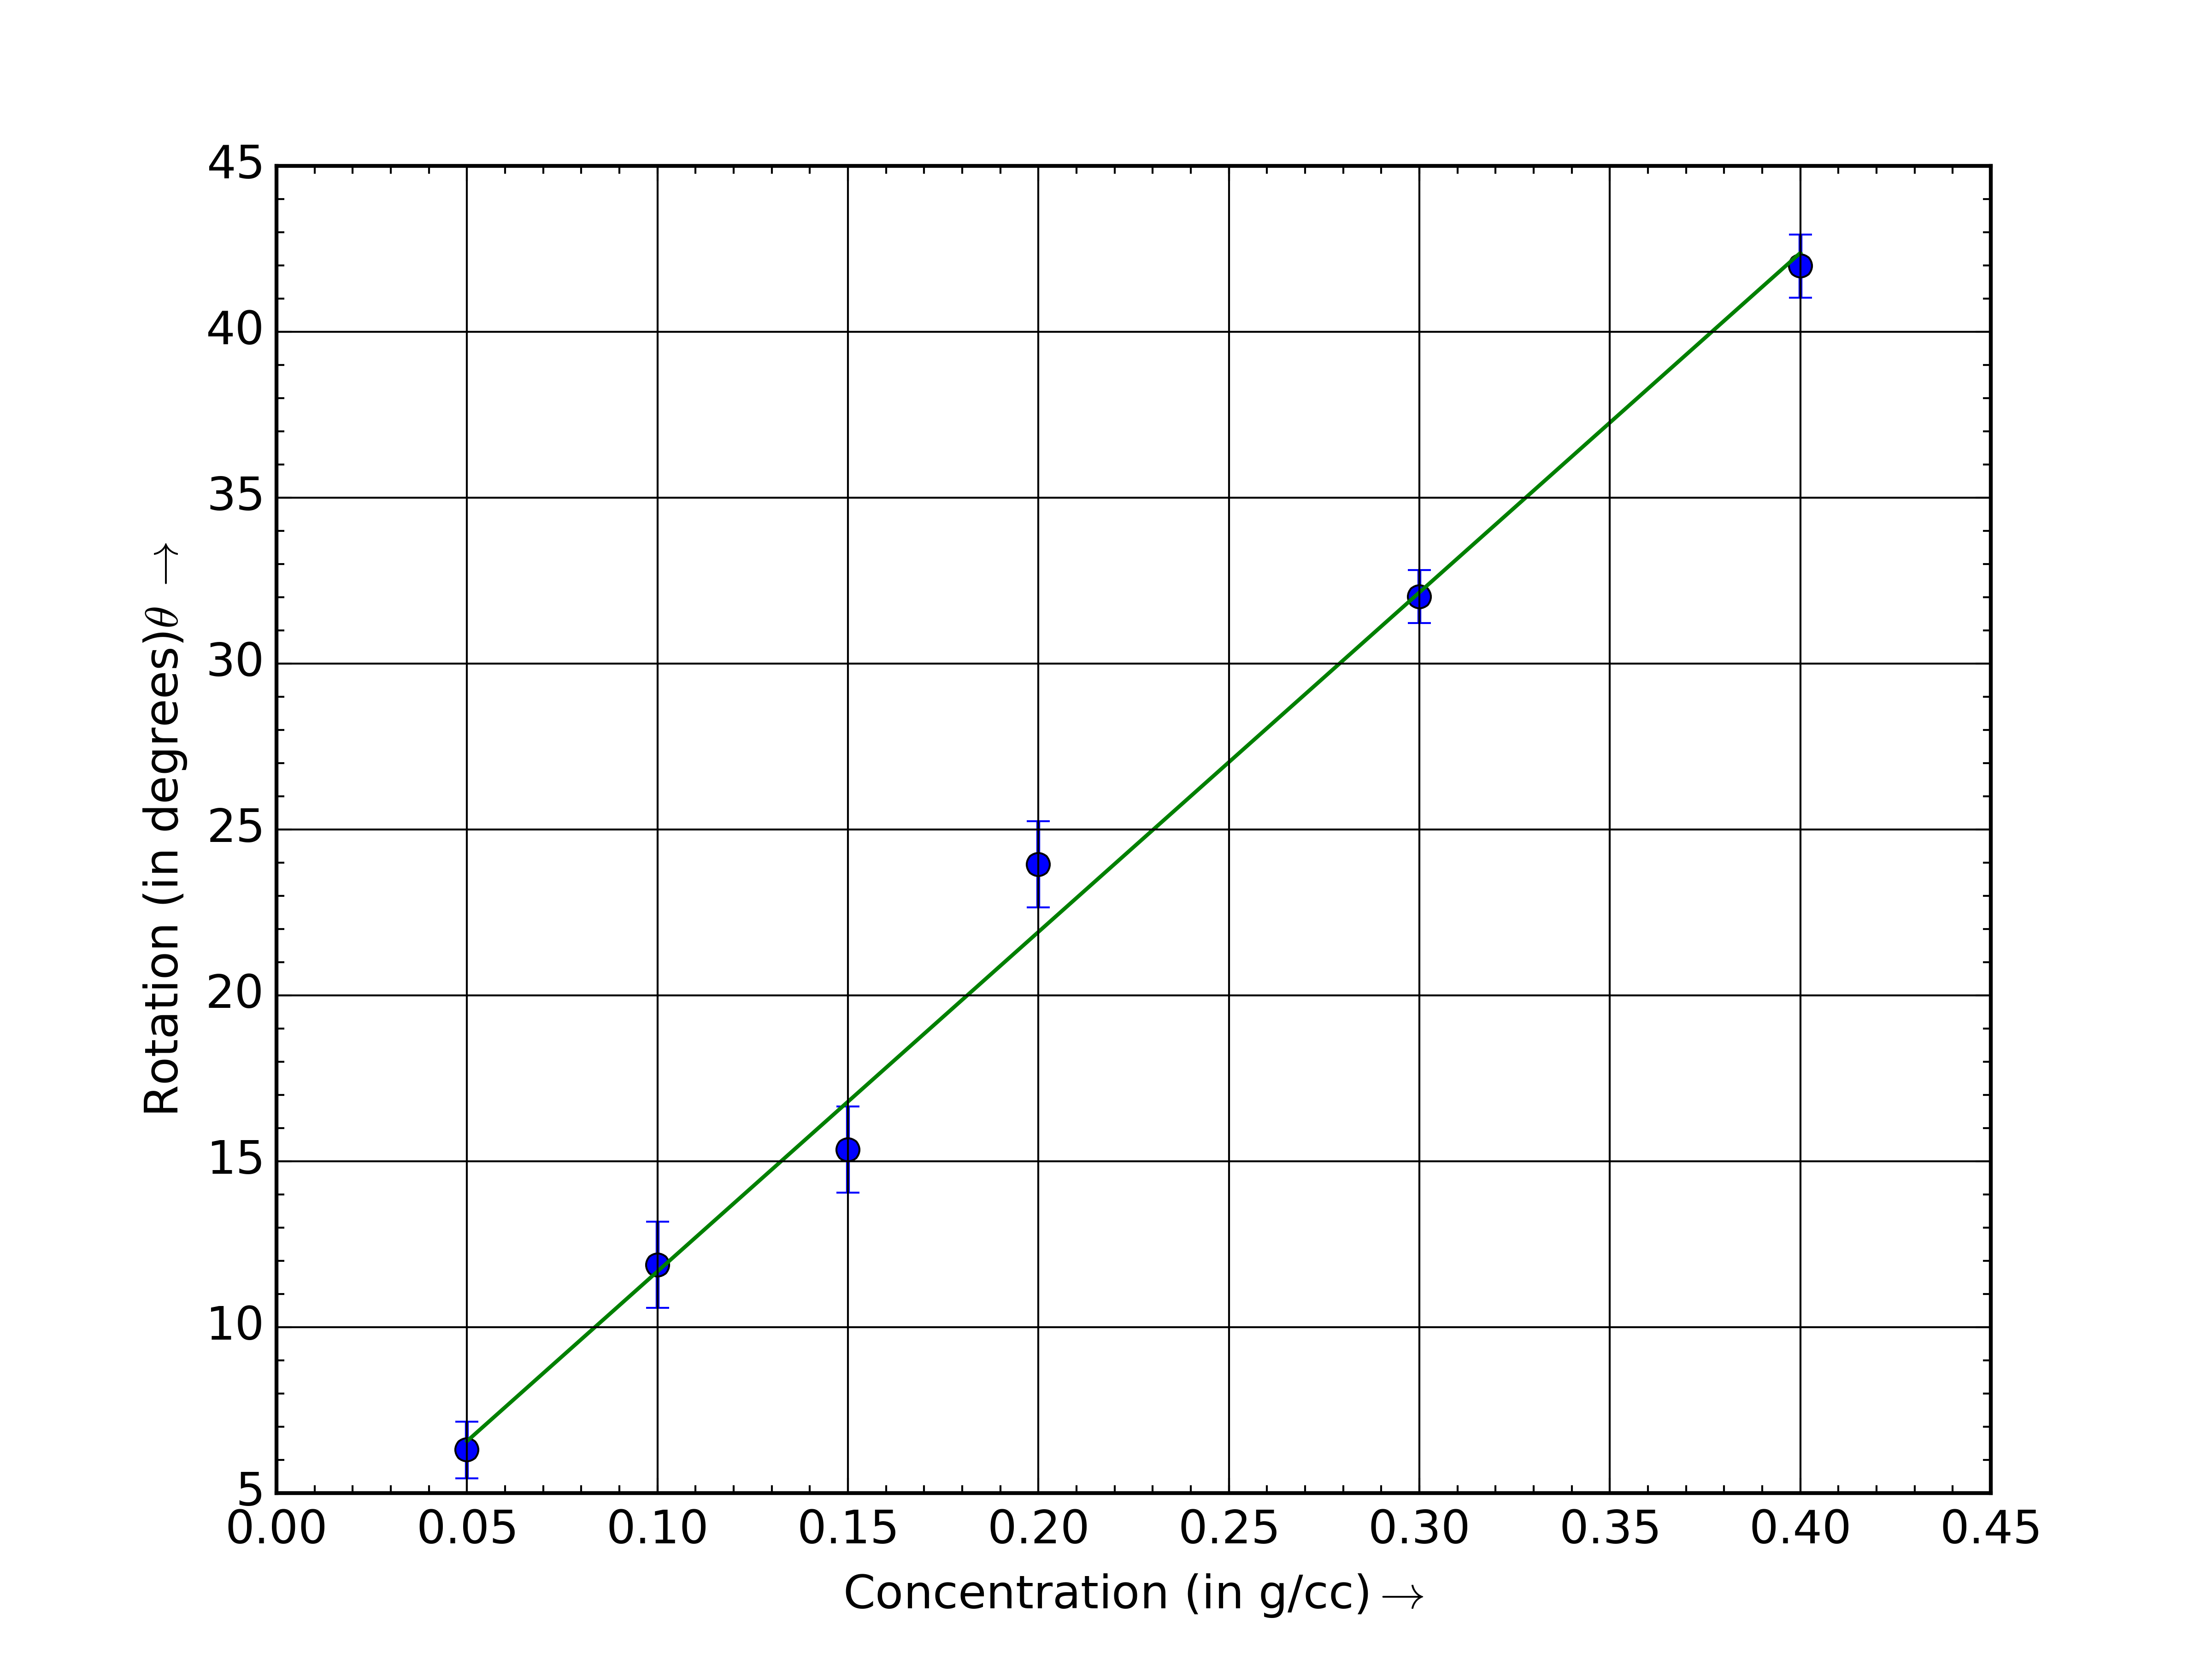
\includegraphics[scale=0.7]{Images/Plot.png}
\caption{Plot of Angle of rotation of polarized light (in degrees) versus concentration (in g/cc)} 
\end{figure}


\subsection{Error analysis}
There are essentially two main sources of error in this experiment:
\begin{enumerate}
\item Error in the concentration due to the error in the weighing scale and the measuring beaker
\item Error in the angle of rotation which, due to the inability of the human eye to perfectly distinguish between equally bright/dark regions and slightly unequal bright/dark regions, will be more than the least count of the instrument
\end{enumerate} 

The slope of the fitted curve is given by:
\begin{align*}
m = \dfrac{n\sum_i c_i \theta_i - (\sum_i c_i)(\sum_i \theta_i)}{n\sum_i c_{i}^{2} -  (\sum_i c_i)^2}
\end{align*}

On differentiating we get an expression for error in terms of the of $(c_i, \theta_i)$ and $\Delta c$ and $\Delta \theta_i$. On substituting the values we will obtain $\Delta m = 0.061 ^{\circ} 100 cc / g$. 

From the relation 
$$S = \dfrac{\theta}{lc} = \dfrac{m}{l}$$
we get, 
\begin{align*}
\implies \dfrac{|\Delta S|}{S}  &= \dfrac{|\Delta m|}{m} + \dfrac{|\Delta l| }{l} \\
&= \dfrac{0.061}{1.023} + \dfrac{0.01}{1.6}\\
&= 0.066
\end{align*}
$$\implies \Delta S =  4.22 \approx 4^{\circ}\ 100 cc / g$$
The error is around 6.6\%. Given this error we can round off $S = 63.93$ to $S = 64$.

\section{Results}
The specific rotation of plane polarized sodium vapor light of wavelength $\lambda = 590\ nm$ and a room temperature of  around 31 $^{\circ}$C using solutions of cane sugar is $(64  \pm 4 ) ^{\circ}\ 100\ cc\ g^{-1}$ . The error margin is around 7\%, which is acceptable considering the sources of error discussed previously. Some more systematic errors in the experiment are given ahead.

 
\section{Precautions and Sources of Error}
\begin{enumerate}
\itemsep0em
\item The optical rotation of a given sample is temperature dependent as well. Ideally the sample must be maintained at a constant temperature;
\item Care should be taken not to tighten the cap of the tube containing the solution too much.  Stressed amorphous substances like glass also show the ability to rotate the plane of polarization;
\item The tube must be rinsed with solution before the solution is poured into it;
\item Only distilled water should be used.
\end{enumerate}

\section{Discussion(optional)}


%-------------------------Bibliography---------------------------------------
\begin{thebibliography}{99}
\bibitem{GA}
Ghatak, Ajoy (2005). Optics (3rd ed.). 

\bibitem{Jha}
Jha, A.K. Textbook of Applied Physics, Volume 1.

% Always cite your sources
\bibitem{DKP} 
\TeX-report. Written in \LaTeXe. Work of Dinesh K. Pinto, St. Stephen's College, 2015.
\end{thebibliography}


\end{document}
